\documentclass[teaching.portfolio.tex]{subfiles}
\begin{document}
This appendix collects a sampling of materials used in recent courses.

\subsection{Sample Syllabus}\hfill\\
Below is a sample syllabus, which will be used for the upcoming Spring 2018 semester.
\begin{center}
  \textsc{Contact Information}
\end{center}

\noindent
\textbf{E-mail:} \href{mailto:farmanb@math.sc.edu}{farmanb@math.sc.edu}\\
\noindent\textbf{Office:} LeConte 317N\\
\noindent\textbf{Office Hours:}
I will be available in my office every Monday/Wednesday, 10:30 am - 12:00 pm.
Additionally, I am available by appointment if these times are not amenable.
You should utilize this time to ask questions about homework, clarify concepts, etc. as needed.\\

\begin{center}
  \textsc{Course Information}
\end{center}

\noindent
\textbf{Lectures:}
Tuesday/Thursday,  10:05 am - 11:20 am in Gambrell, Room 103.\\

\noindent\textbf{Learning Outcomes:} A student who successfully completes Calculus II (MATH 142) should continue to develop as an independent learner 
with the ability to approach problems from a conceptual viewpoint, to utilize more than one idea in a single problem, and to apply appropriate 
calculus skills to problems in context.

In particular, the successful student will master concepts and gain skills needed to solve problems related to 
techniques of integration, 
improper integrals, 
applications of integration, 
convergence of sequences and series,
power series,
Taylor and Maclaurin series,
applications of Taylor polynomials,
polar coordinates,
area and length in polar coordinates.\\

\noindent\textbf{Pre-Requisites:} Qualification through placement or a grade of C or better in MATH 141.\\

\noindent\textbf{Text:}
The required text for this course is\\
\begin{center}
  {\it Thomas' Calculus: Early Transcendentals}, $13^{\text{th}}$ Edition, Thomas, Weir, Hass, 2013.  \\ISBN 9781323157138.
\end{center}

\noindent
The university bookstore offers two options for obtaining this text:
\begin{itemize}
\item
  A bundle that includes a hard copy of the text and a MyMathLab access key,
\item
  A MyMathLab access key that grants access to a digital copy of the text.
\end{itemize}
You may choose either option, however, be aware that it is {\bf expected} that you will read the text outside of lecture.
In making your choice, be sure that you choose an option that you will read.\\

\noindent\textbf{Course Website:} The URL for the course website is
\begin{center}
  \url{http://people.math.sc.edu/farmanb/courses/142/S18/index.html}
\end{center}
Here you can find a digital copy of the syllabus, lecture notes, test dates, and other various announcements.

\begin{center}
  \textsc{Coursework}
\end{center}
\noindent
\textbf{Homework:}
Homework assignments are available on MyMathLab.
All MyMathLab homework assignments are currently available and may be accessed using the class key
\begin{center}
  {\bf farman\#\#\#\#\#}
\end{center}
It is important that you create a MyMathLab account and register for the course as soon as possible.

The assignments are separated into three groups corresponding to the material on each of the exams.
The problems are chosen to highlight the core concepts on each exam and mastery of these homework sets serve as a good indicator for exam performance.
As such, you should ensure that you fully understand the material on these homework sets; that is, upon completion of the homework set, you should be capable of completing similar problems without the aid of the text or the various tools provided by MyMathLab.

The homework sets in each group are due the day before the corresponding exam.
Late work will {\bf not} be accepted, and you are solely responsible for ensuring that these assignments are completed on time.
These assignments are relatively long, so you should be working through them as we cover the material.
Do {\bf not} leave these assignments until the last minute.\\

\noindent\textbf{Exams:}
There will be three in-class exams.
The exams are tentatively scheduled as follows:
\begin{center}
  \begin{tabular}{ll}
    Exam 1: & Thursday, February 15, 2018,\\
    Exam 2: & Thursday, March 22, 2018,\\
    Exam 3: & Thursday, April 19, 2018.\\
  \end{tabular}\\
\end{center}
Though unexpected, any deviations from this schedule will be announced during lecture and reflected on the course website.\\

\noindent\textit{Missed Assessments:}
There will {\bf not} be any make-up exams or quizzes.
If you miss one exam, your final exam grade will replace the missing exam grade.
\textbf{This policy is intended only for exams missed due to illness, accidents, etc.  
  It does NOT mean that your lowest exam grade will be dropped.}
Any further missed exams will receive a grade of zero.\\

\noindent\textbf{Final Exam:} There will be a cumulative final exam on Tuesday, May 8, 2018 at 9:00 am.
The date and time of the final exam is determined by the registrar and \textbf{may not be changed} except under extreme circumstances.\\

\textbf{Scheduling your travel home before the day of the final exam does not constitute a valid excuse for rescheduling the final exam.}
Failure to appear at the final exam will result in a zero on the final exam.

\begin{center}
  \textsc{Grading}
\end{center}
\textbf{Scale:}
Grades will be assigned on the following scale:
\begin{center}
  \begin{tabular}{ll}
    A: &90-100\%,\\
    B: & 80-89\%,\\
    C: & 70-79\%,\\
    D: & 60-69\%,\\
    F: & $<$ 60\%.\\
  \end{tabular}\\
\end{center}
\textbf{Weights:}
Final grades will be calculated with the following weights:
\begin{center}
  \begin{tabular}{lr}
    Homework: & 30\%,\\
    Quizzes: &10\%,\\
    Exams: & 30\%,\\
    Final Exam: & 30\%.\\
  \end{tabular}\\
\end{center}

\begin{center}
  \textsc{Tutoring Center}
\end{center}
\noindent
The mathematics department at the University of South Carolina offers free tutoring to UofSC students in LeConte 105.
It is staffed with talented graduate students who will answer questions about MATH 111, 115, 122, 141, 142, and 170.
No appointment is necessary--just stop by during the hours listed on the schedule at
\begin{center}
  \url{http://math.sc.edu/math-tutoring-center}.
\end{center}

\begin{center}
  \textsc{Student Success Center}
\end{center}
\noindent
In partnership with UofSC faculty, the Student Success Center (SSC) offers a number of programs to assist you in better understanding your course material and to aid you on your path to success. 
SSC programs are facilitated by professional staff, graduate students, and trained undergraduate peer leaders who have previously excelled in their courses.
Resources available to students include: 
\begin{itemize}
\item 
  \textbf{Peer Tutoring:} make a one-on-one appointment with a Peer Tutor by going to \url{http://www.sc.edu/success}. 
  If a course is not on the semester’s supported-course list, there is a process for requesting assistance. 
  The full schedule of days/times/locations for drop-in and Online Tutoring hours can also be viewed on the SSC website.
\item
  \textbf{Supplemental Instruction (SI):} attend SI Sessions to focus on the most difficult content being covered in class. 
  SI Leaders are assigned to specific sections of courses and hold three weekly study sessions that can serve as “built-in study time.” 
  The schedule is posted on the SSC website each week and will also be communicated by the SI Leader.
\item
  \textbf{Peer Success Consultations:} make a one-on-one Success Consultation with a Peer Consultant to work on developing study skills, setting goals, and connecting to a variety of campus resources. 
  Your instructor may communicate with the SSC via Success Connect, an online referral system, regarding your progress in the course. 
  If contacted by the SSC, please schedule a Success Consultation. 
  Success Connect referrals are not punitive and any information shared by your professor is confidential and subject to FERPA regulations.
\end{itemize}
SSC services are offered to all UofSC undergraduates at no additional cost.
You are invited to call the Student Success Hotline at (803) 777-1000, visit \url{http://www.sc.edu/success}, or come to the SSC in the Thomas Cooper Library (Mezzanine Level) to check schedules and make appointments. 

\begin{center}
  \textsc{Expectations}
\end{center}

\noindent
\textbf{Academic Integrity:} 
\textit{As a Carolinian...I will practice personal and academic integrity.}\\

\noindent 
The University of South Carolina expects high standards in all areas from its students.
The University, as well as the faculty, staff, alumni, and students believe strongly in the Honor Code.
This Code requires acceptance of certain responsibilities and agreement by all students to abide by the spirit of the Honor Code upon entering the University of South Carolina.
In order that you may better understand the required responsibilities, the general University community codes are outlined below.

\begin{enumerate}
\item
  It shall be the responsibility of every faculty member, student, administrator and staff member of the University community to uphold and maintain the academic standards and integrity of the University of South Carolina.
\item
  Any member of the University community, who has reasonable grounds to believe that an infraction of the Honor Code has occured, has an obligation to report the alleged violation.
  Violation of any of the following standards subjects the student to disciplinary action: improper collaboration, cheating, lying, bribery, and plagiarism.
\end{enumerate}

\noindent
Your enrollment in this class signifies your willingness to accept these responsibilities and uphold the Honor Code of the University of South Carolina.
Please review the Honor Code via
\begin{center}
  \url{http://www.sa.sc.edu/academicintegrity/}.
\end{center}

\noindent
Any deviation from this expectation \textbf{will result in a grade of F in the course} and disciplinary action through the Office of Academic Integrity.\\

\noindent\textbf{Attendance:} 
Students are obligated to complete all assigned work promptly, to attend class regularly, and to participate in whatever class discussion may occur.\\

\noindent
The following events or circumstances are potentially excusable absences:
\begin{itemize}
\item
  participation in an authorized University activity (such as musical performances, academic competitions, or varsity athletic events in which the student plays a formal role in a University sanctioned event),
\item
  required participation in military duties,
\item
  mandatory admission interviews for professional or graduate school which cannot be rescheduled,
\item
  participation in legal proceedings or administrative duties that require a student's presence,
\item
  death or major illness in a student’s immediate family,
\item
  illness of a dependent family member
\item
  religious holy day if listed on \url{http://www.interfaithcalendar.org},
\item
  illness that is too severe or contagious for the student to attend class,
\item
  weather-related emergencies.
\end{itemize}
For more information, see the University Attendance Policy:
\begin{center}
  \url{http://bulletin.sc.edu/content.php?catoid=66&navoid=1813#Attendance_Policy}
\end{center}
\subsection{Sample Exam}
The following is an exam given to my Calculus II class in July 2014.
\begin{thm}
  Find the volume of the solid obtained by rotating the region bounded by the curves $f(x) = 4(x - 2)^2$ and $g(x) = x^2 - 4x + 7$ about the $y$-axis.
\end{thm}

\textbf{Integration}\\

\noindent For each of the following problems, decide which method of integration is appropriate and compute the given integrals.
If you need more space for a problem, use the back of the page and indicate that you have done so.

\begin{thm}
  Compute $\displaystyle{\int\sin^3(\theta)\cos^2(\theta)d\theta}$.
\end{thm}

\begin{thm}
  Compute $\displaystyle{\int \frac{\ln(x)}{x^2}dx}$.
\end{thm}

\begin{thm}
  Compute $\displaystyle{\int\frac{dx}{x^2\sqrt{x^2-9}}}$.
\end{thm}

\begin{thm}
  Compute $\displaystyle{\int\frac{x}{x^2 - 5x + 6}}dx$.
\end{thm}

\begin{thm}
  Explain why $\displaystyle{\int_0^3 \frac{dx}{\sqrt{x}}}$ is an improper integral, then evaluate it.
\end{thm}

\textbf{Series and Sequences}
\begin{thm}
  Express $5.\overline{5} = 5.55555\ldots$ as a rational number. [Hint: Geometric Series.]
\end{thm}

\noindent
Test the following series for convergence.
You may use any of the tests we covered in class, however you {\bf must indicate which test you use}.
\begin{thm}
  $\displaystyle{\sum_{k=1}^\infty \frac{2^k k!}{(k+2)!}}.$
\end{thm}

\begin{thm}
  $\displaystyle{\sum_{n=1}^\infty \frac{2^{2n}}{n^n}}$
\end{thm}

\textbf{Power Series}

\begin{thm}
  Find the Taylor expansion of $\ln(x)$ about $a = 2$.
  Find the radius of convergence and the interval of convergence for the series you find.
\end{thm}

\textbf{Bonus}

\begin{thm}
  Sketch the curve with polar equation $\displaystyle{r = \sin^2(2\theta)}$.
\end{thm}
\subsection{Sample Course Notes}
Below is a sample of lecture notes generated for Math 122: Calculus for Business Administration and Social Sciences taught in Spring 2017.
This course presented a striking and unusual challenge as a calculus instructor: teaching limits and continuity is forbidden.
As a result, it became clear that generating animations and detailed lecture notes with pictures and heuristic explanations for topics such as integration would be necessary to motive the formal manipulations the students were asked to perform.
Since the animations are not easily embedded in the beamer handout, they have been removed from the slides and links are provided below:
\begin{itemize}
\item
  Right Error:
  \begin{center}
    \url{http://people.math.sc.edu/farmanb/courses/122/gifs/errorRight.gif}
  \end{center}
\item
  Left Error:
  \begin{center}
    \url{http://people.math.sc.edu/farmanb/courses/122/gifs/errorLeft.gif}
  \end{center}
\item
  Right Estimate:
  \begin{center}
    \url{http://people.math.sc.edu/farmanb/courses/122/gifs/rightEstimate.gif}
  \end{center}
\item
  Left Estimate:
  \begin{center}
    \url{http://people.math.sc.edu/farmanb/courses/122/gifs/leftEstimate.gif}
  \end{center}
\end{itemize}
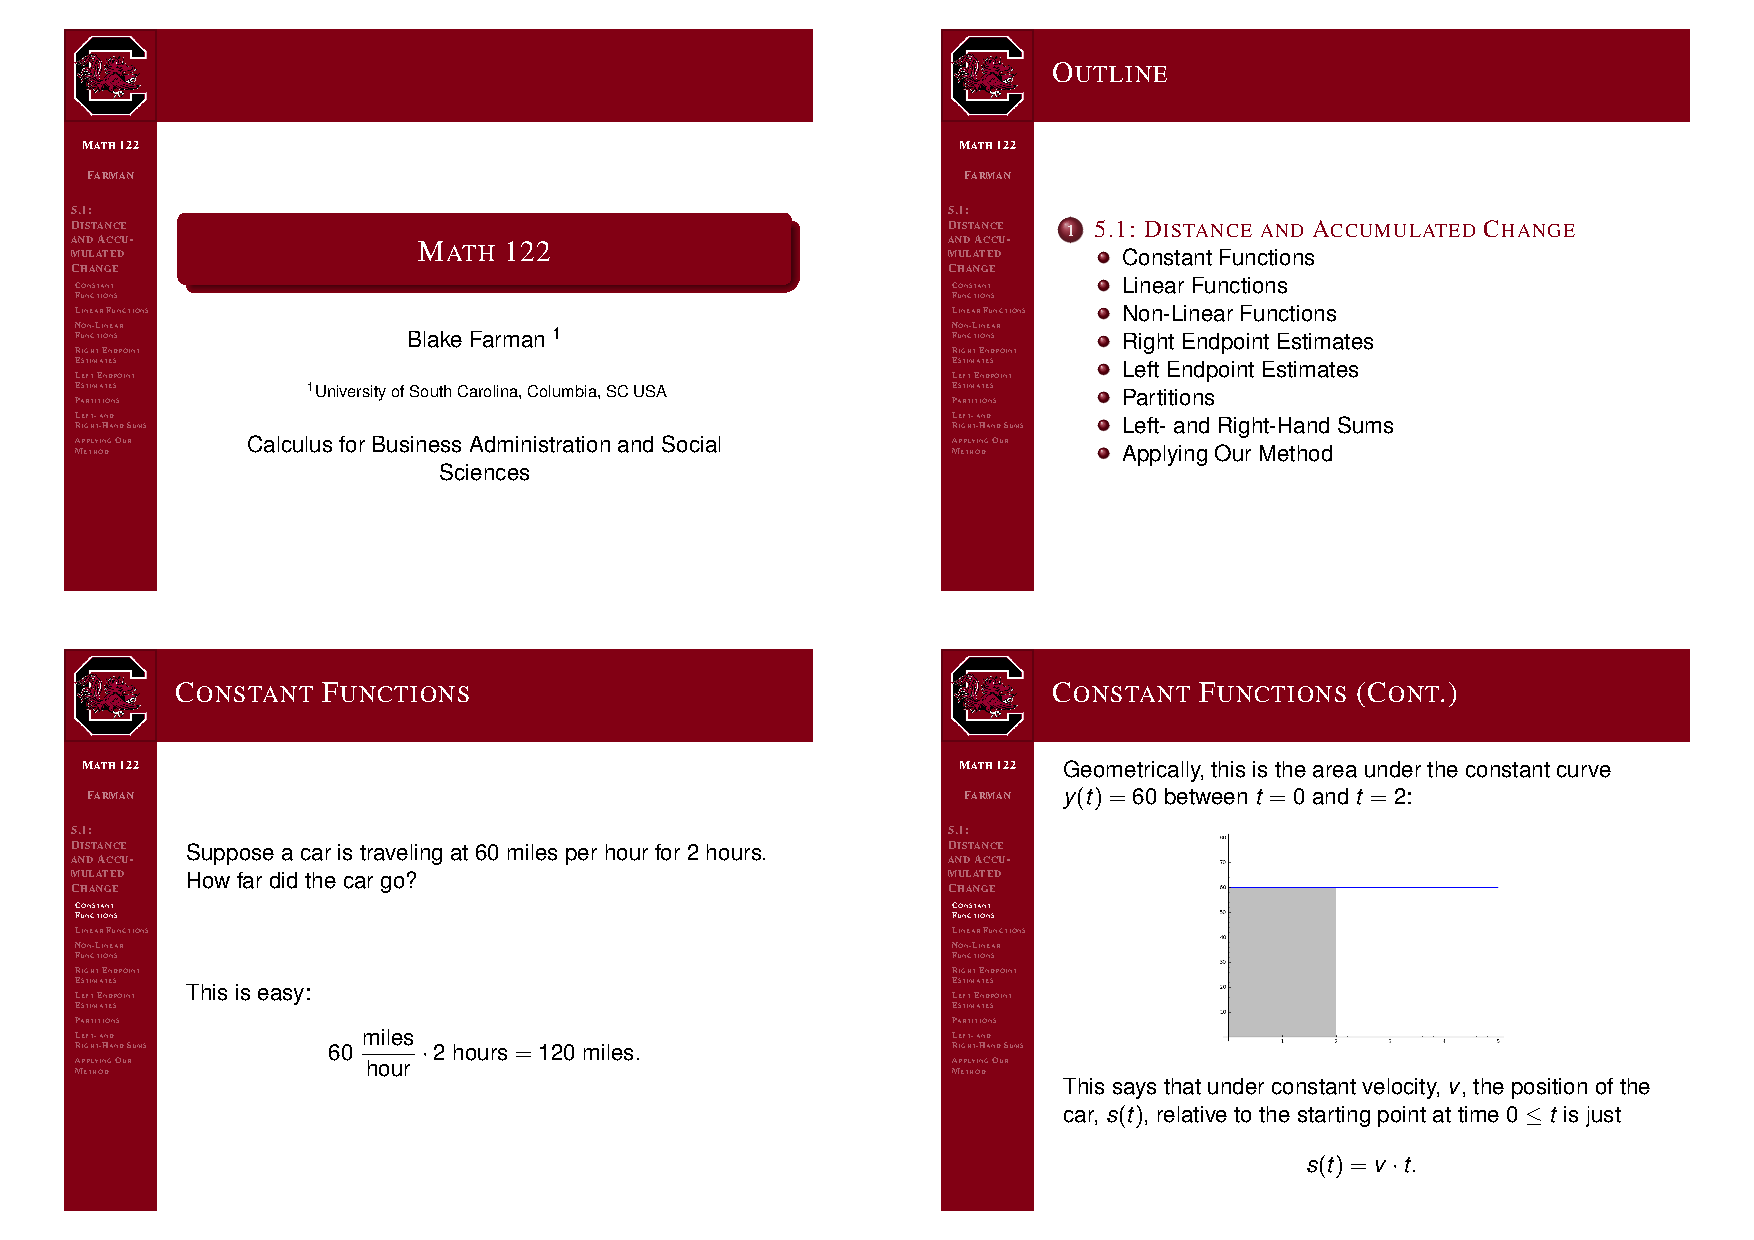
\includepdf[pages=-]{../notes/122-integrals.pdf}
\end{document}

